\documentclass[12pt]{beamer}
\input{../Preambulos/preambulo_Beamer_Madrid_whale}
\usepackage{../Estilos/BeamerFC}
\usepackage{../Estilos/ColoresLatex}
\input{../Preambulos/pre_codigo}
\usepackage[siunitx]{circuitikz}
\usepackage{parskip}
\usetikzlibrary{arrows,patterns,shapes}
\usetikzlibrary{decorations.markings}
\usetikzlibrary{arrows}
\usepackage{blkarray}

\DeclareSIUnit\megapascal{\mega\pascal}
% \usefonttheme{serif}

\title{\large{Problemas de eigenvalores con matrices simétricas}}
\subtitle{Tema 4 - Álgebra matricial}
\author{M. en C. Gustavo Contreras Mayén}
\date{}

\begin{document}
\maketitle

\section*{Contenido}
\frame{\tableofcontents[currentsection, hideallsubsections]}


\section{Problemas de eigenvalores}
\frame{\tableofcontents[currentsection, hideothersubsections]}
\subsection{Introducción}

\begin{frame}
\frametitle{Introducción}
Nuestro punto de partida es el siguiente:
\\
\bigskip
\pause
Encontrar $\lambda$ para el cual existe una solución no trivial de:
\begin{align*}
\mathbf{A \; x} = \lambda \; \mathbf{x}
\end{align*}
\end{frame}
\begin{frame}
\frametitle{Definiendo la forma estándar}
La \textbf{\textcolor{lava}{forma estándar}} de un problema matricial de eigenvalores es:
\pause
\begin{align}
\mathbf{A \; x} = \lambda \mathbf{x}
\label{eq:ecuacion_09_01}
\end{align}
donde $\mathbf{A}$ es una matriz dada de tamaño $n \times n$. \pause El problema que debemos resolver, es calcular un escalar $\lambda$ y un vector $\mathbf{x}$.
\end{frame}
\begin{frame}
\frametitle{Escribiendo el problema como un sistema de ecs.}
Reescribimos la ecuación (\ref{eq:ecuacion_09_01}) de la forma:
\pause
\begin{align}
\big( \mathbf{A} - \lambda \; \mathbf{I} \big) \mathbf{x} = \mathbf{0}
\label{eq:ecuacion_09_02}
\end{align}
Se hace evidente que se trata de un sistema de $n$ ecuaciones homogéneas.
\end{frame}
\begin{frame}
\frametitle{Las soluciones del sistema de ecs.}
Una solución obvia es la trivial $x = 0$. \pause Una solución no trivial sólo puede existir si el determinante de la matriz de coeficientes es nulo, es decir:
\pause
\begin{align}
\abs{ \mathbf{A} - \lambda \; \mathbf{I} } = \mathbf{0}
\label{eq:ecuacion_09_03}
\end{align}
\end{frame}
\begin{frame}
\frametitle{Ecuación característica}
La expansión del determinante nos lleva a la ecuación polinomial, también conocida como la \textbf{\textcolor{ao}{ecuación característica}}:
\pause
\begin{align*}
a_{0} + a_{1} \; \lambda + a_{2} \; \lambda^{2} + \ldots + a_{n} \; \lambda^{n} = 0
\end{align*}
\end{frame}
\begin{frame}
\frametitle{Eigenvalores y eigenvectores}
Que tiene las raíces $\lambda_{i} \; i = 1, 2, \ldots,  n$, llamados \textbf{\textcolor{armygreen}{eigenvalores}} de la matriz $\mathbf{A}$.
\\
\medskip
\pause
Las soluciones $x_{i}$ de $(\mathbf{A}- \lambda_{i} \; \mathbf{I}) \mathbf{x} = \mathbf{0}$ son conocidas como \textbf{\textcolor{brickred}{eigenvectores}}.
\end{frame}
\begin{frame}
\frametitle{Ejemplo}
Consideremos la matriz:
\pause
\begin{align}
\mathbf{A} = \begin{bmatrix}
1 & -1 & 0 \\
-1 & 2 & -1 \\
0 & -1 & 1
\end{bmatrix}
\label{eq:ecuacion_09_a}
\end{align}
\end{frame}
\begin{frame}
\frametitle{Ecuación característica}
La ecuación característica es:
\pause
\begin{align}
\abs{ \mathbf{A} - \lambda \; \mathbf{I} }=  \begin{vmatrix}
1 - \lambda & -1 & 0 \\
-1 & 2 - \lambda & -1 \\
0 & -1 & 1 - \lambda
\end{vmatrix} 
= -3 \lambda +  4 \lambda^{2} - \lambda^{3} = 0
\label{eq:ecuacion_09_b}
\end{align}
\pause
Las raíces de esta ecuación son $\lambda_{1} = 0$, $\lambda_{2} = 1$, $\lambda_{3} = 3$.
\end{frame}
\begin{frame}
\frametitle{Recuperando los eigenvectores}
Para calcular el eigenvector correspondiente a $\lambda_{3}$, \pause sustituimos $\lambda = \lambda_{3}$ en la ecuación (\ref{eq:ecuacion_09_02}), para obtener:
\pause
\begin{align}
\begin{bmatrix}
-2 & -1 & 0 \\
-1 & -1 & -1 \\
0 & -1 & -2
\end{bmatrix}
\begin{bmatrix}
x_{1} \\
x_{2} \\
x_{3} 
\end{bmatrix} = 
\begin{bmatrix}
0 \\
0 \\
0
\end{bmatrix}
\label{eq:ecuacion_09_c}
\end{align}
\end{frame}
\begin{frame}
\frametitle{El determinante de la matriz}
Sabemos que el determinante de la matriz de coeficientes es cero, de modo que las ecuaciones no son linealmente independientes. 
\\
\bigskip
\pause
Por lo tanto, podemos asignar un valor arbitrario a cualquier componente de $x$ y usar dos de las ecuaciones para calcular los otros dos componentes.
\end{frame}
\begin{frame}
\frametitle{Ocupando un valor arbitrario}
Escogiendo $x_{1} = 1$, la primera ecuación de la ecuación (\ref{eq:ecuacion_09_c}) nos devuelve $x_{2} = -2$, y de la tercera ecuación se obtiene $x_{3} = 1$. 
\\
\bigskip
\pause
Así, el vector propio asociado con $\lambda_{3}$ es:
\pause
\begin{align*}
\mathbf{x}_{3}  = \begin{bmatrix}
1 \\
-2 \\
1
\end{bmatrix}
\end{align*}
\end{frame}
\begin{frame}
\frametitle{Recuperando los otros dos eigenvectores}
Obtenemos los otros dos eigenvectores de la misma forma:
\pause
\begin{align*}
\mathbf{x}_{2} = \begin{bmatrix}
1 \\
0 \\
-1
\end{bmatrix} \hspace{1cm}
\mathbf{x}_{1} =  \begin{bmatrix}
1 \\
1 \\
1
\end{bmatrix}
\end{align*}
\end{frame}
\begin{frame}
\frametitle{Notación de utilidad}
A veces es conveniente mostrar los eigenvectores como columnas de una matriz $\mathbf{X}$. \pause Para nuestro primer ejemplo, esta matriz es:
\pause
\begin{align*}
\mathbf{X} = \left[ \mathbf{x}_{1} \hspace{0.3cm} \mathbf{x}_{2} \hspace{0.3cm} \mathbf{x}_{3} \right] = 
\begin{bmatrix}
1 & 1 & 1 \\
1 & 0 & -2 \\
1 & -1 & 1
\end{bmatrix}
\end{align*}
\end{frame}
\begin{frame}
\frametitle{Magnitud del eigenvector}
De este ejemplo se desprende claramente que la magnitud de un eigenvector es indeterminada; sólo su dirección se puede calcular a partir de la ecuación (\ref{eq:ecuacion_09_02}).
\\
\bigskip
\pause
Es costumbre \textbf{\textcolor{cadetblue}{normalizar}} los eigenvectores asignando una magnitud unitaria a cada vector. 
\end{frame}
\begin{frame}
\frametitle{Eigenvectores normalizados}
Así, los eigenvectores normalizados en nuestro ejemplo son:
\pause
\begin{align*}
\mathbf{X} = \begin{bmatrix}
1 / \sqrt{3} & 1 / \sqrt{2} & 1 / \sqrt{6} \\
1 / \sqrt{3} & 0 & -2 / \sqrt{6} \\
1 / \sqrt{3} & -1 / \sqrt{2} & 1 / \sqrt{6}
\end{bmatrix}
\end{align*}
\pause
\textbf{Nota:} A lo largo del tema supondremos que los eigenvectores están normalizados.
\end{frame}
\begin{frame}
\frametitle{Propiedades de los eigevalores y eigenvectores}
Mencionaremos algunas propiedades útiles de los eigenvalores y de los eigenvectores (dados sin prueba):
\setbeamercolor{item projected}{bg=champagne,fg=chestnut}
\setbeamertemplate{enumerate items}{%
\usebeamercolor[bg]{item projected}%
\raisebox{1.5pt}{\colorbox{bg}{\color{fg}\footnotesize\insertenumlabel}}%
}
\begin{enumerate}[<+->]
\item Todos los eigenvalores de una matriz simétrica son reales.
\item Todos los eigenvalores de una matriz simétrica definida positiva son reales y positivos.
\seti
\end{enumerate}
\end{frame}
\begin{frame}
\frametitle{Propiedades de los eigevalores y eigenvectores}
\setbeamercolor{item projected}{bg=champagne,fg=chestnut}
\setbeamertemplate{enumerate items}{%
\usebeamercolor[bg]{item projected}%
\raisebox{1.5pt}{\colorbox{bg}{\color{fg}\footnotesize\insertenumlabel}}%
}
\begin{enumerate}[<+->]
\conti
\item Los eigenvectores de una matriz simétrica son ortonormales; Es decir, $\mathbf{X}^{T} \; \mathbf{X} = \mathbf{I}$.
\item Si los eigenvalores de $\mathbf{A}$ son $\lambda_{i}$, entonces los eigenvalores de $\mathbf{A}^{-1}$ son $\lambda_{i}^{-1}$
\end{enumerate}
\end{frame}
\begin{frame}
\frametitle{Naturaleza de los problema de eigenvalores}
Los problemas de eigenvalores que se originan a partir de problemas físicos a menudo terminan con una matriz $\mathbf{A}$ simétrica.
\\
\bigskip
\pause
Esto es afortunado de cierta manera, porque los problemas simétricos de los eigenvalores son más fáciles de resolver que sus homólogos no simétricos (que pueden tener eigenvalores complejos).
\end{frame}
\begin{frame}
\frametitle{Naturaleza de los problema de eigenvalores}
A lo largo del Tema 4, consideraremos a los eigenvalores y eigenvectores de matrices simétricas.
\\
\bigskip
\pause
Es común encontrar problemas de eigenvalores en el análisis de las vibraciones y la estabilidad.
\end{frame}
\begin{frame}
\frametitle{Naturaleza de los problema de eigenvalores}
Estos problemas a menudo tienen las siguientes características:
\setbeamercolor{item projected}{bg=crimson,fg=cream}
\setbeamertemplate{enumerate items}{%
\usebeamercolor[bg]{item projected}%
\raisebox{1.5pt}{\colorbox{bg}{\color{fg}\footnotesize\insertenumlabel}}%
}
\begin{enumerate}[<+->]
\item Las matrices son grandes y escasas - \emph{sparse} -(por ejemplo, tienen una estructura en bandas).
\item Necesitamos conocer sólo los eigenvalores; si se requieren eigenvectores, sólo unos cuantos de ellos son de interés.
\end{enumerate}
\end{frame}
\begin{frame}
\frametitle{Procedimiento para calcular los eigevalores}
Un algortimo útil de eigenvalores, debe ser capaz de utilizar estas características para minimizar los cálculos.
\\
\bigskip
\pause
En particular, debe ser lo suficientemente flexible como para calcular sólo lo que necesitamos y no más.
\end{frame}
\begin{frame}
\frametitle{Ejemplo}
Considera el siguiente sistema:
\\
\bigskip
\pause
\begin{figure}
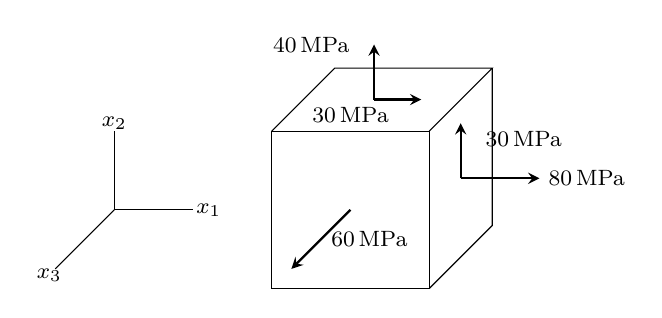
\begin{tikzpicture}[font=\footnotesize]
    \draw(0, 0) -- (1, 0) node [near end, pos=1.2] {$x_{1}$};
    \draw(0, 0) -- (0, 1) node [near end, pos=1.1] {$x_{2}$};
    \draw(0, 0) -- (-0.75, -0.75) node [near end, pos=1.1] {$x_{3}$};

    \draw (2, -1) rectangle (4, 1);
    \draw (2, 1) -- (2.8, 1.8) -- (4.8, 1.8) -- (4, 1);
    \draw (4, -1) -- (4.8, -0.2) -- (4.8, 1.8);

    
    \draw [-stealth, thick] (3, 0) -- (2.25, -0.75) node [midway, right] {$\SI{60}{\mega\pascal}$};
    \draw [-stealth, thick] (4.4, 0.4) -- (5.4, 0.4);
    \node at (6, 0.4) {$\SI{80}{\mega\pascal}$};
    \draw [-stealth, thick] (4.4, 0.4) -- (4.4, 1.1);
    \node at (5.2, 0.9) {$\SI{30}{\mega\pascal}$};
    \draw [-stealth, thick] (3.3, 1.4) -- (3.9, 1.4);
    \node at (3, 1.2) {$\SI{30}{\mega\pascal}$};
    \draw [-stealth, thick] (3.3, 1.4) -- (3.3, 2.1);
    \node at (2.5, 2.1) {$\SI{40}{\mega\pascal}$};
\end{tikzpicture}
\end{figure}
\end{frame}
\begin{frame}
\frametitle{Matriz de esfuerzo}
La matriz de esfuerzo (tensor) que corresponde al estado que se mostró en la figura anterior es:
\pause
\begin{align*}
\mathbf{S} = 
\begin{bmatrix}
80 & 30 & 0 \\
30 & 40 & 0 \\
0 & 0 & 60
\end{bmatrix}
\, \text{MPa}
\end{align*}
\end{frame}
\begin{frame}
\frametitle{Componentes de la matriz}
Ccada fila de la matriz consta de los tres componentes de tensión que actúan en un plano de coordenadas.
\\
\bigskip
\pause
Se puede demostrar que los eigenvalores de $\mathbf{S}$ son las tensiones principales y que los eigenvectores son normales a los planos principales. \pause \textbf{Determina las tensiones principales y los vectores propios}.
\end{frame}
\begin{frame}
\frametitle{Solución al problema}
La ecuación característica $\abs{\mathbf{S} - \lambda \, \mathbf{I}} = \mathbf{0}$ es:
\pause
\begin{align*}
\mdet{
80 - \lambda & 30 & 0 \\
30 & 40 - \lambda & 0 \\
0 & 0 & 60 - \lambda
} = 0
\end{align*}
\end{frame}
\begin{frame}
\frametitle{Desarrollando el determinante}
Expandiendo el determinante, se obtiene:
\pause
\begin{align*}
(60 - \lambda) \big[ (80 - \lambda) (40 - \lambda) - 900 \big] &= 0 \\[0.5em]
(60 - \lambda) (\lambda^{2} - 120 \, \lambda + 2300) &= 0
\end{align*}
\pause
que nos devuelve las tensiones principales:
\pause
\begin{align*}
\lambda_{1} = \SI{23.944}{\mega\pascal} \hspace{1.2cm} \lambda_{2} = \SI{60}{\mega\pascal} \hspace{1.2cm} \lambda_{3} = \SI{96.056}{\mega\pascal}
\end{align*}
\end{frame}
\begin{frame}
\frametitle{Solución con $\lambda_{1}$}
El primer eigenvector es solución de $(\mathbf{S} - \lambda_{1} \mathbf{I}) \mathbf{x} = 0$, de manera equivalente:
\pause
\begin{align*}
\begin{bmatrix}
56.056 & 30.0 & 0 \\
30.0 & 16.056 & 0 \\
0 & 0 & 36.056
\end{bmatrix}
\begin{bmatrix}
x_{1} \\
x_{2} \\
x_{3}
\end{bmatrix}
= \begin{bmatrix}
0 \\
0 \\
0
\end{bmatrix}
\end{align*}
\end{frame}
\begin{frame}
\frametitle{Eligiendo $x_{1}$}
Eligiendo $x_{1} = 1$, \pause se obtiene:
\pause
\begin{eqnarray*}
\begin{aligned}
x_{2} &= - \dfrac{56.056}{30} = - 1.8685 \\ \pause
x_{3} &= 0
\end{aligned}
\end{eqnarray*}
\pause
Por lo que el vector normalizado es:
\pause
\begin{align*}
\mathbf{x}_{1} = \big[ 0.4719 \quad -0.8817 \quad 0 \big]^{T}
\end{align*}
\end{frame}
\begin{frame}
\frametitle{Solución con $\lambda_{2}$}
El segundo eigenvector se obtiene de $(\mathbf{S} - \lambda_{2} \mathbf{I}) \mathbf{x} = 0$:
\pause
\begin{align*}
\begin{bmatrix}
20 & 30 & 0 \\
30 & -20 & 0 \\
0 & 0 & 0
\end{bmatrix}
\begin{bmatrix}
x_{1} \\
x_{2} \\
x_{3}
\end{bmatrix}
= \begin{bmatrix}
0 \\
0 \\
0
\end{bmatrix}
\end{align*}
\end{frame}
\begin{frame}
\frametitle{Eligiendo $x_{2}$}
Esta ecuacion se satisface con $x_{1} = x_{2}$ y para cualquier valor de $x_{3}$.
\\
\bigskip
\pause
Escogiendo $x_{3} = 1$, el eigenvector es:
\pause
\begin{align*}
\mathbf{x}_{2} = \big[ 0 \quad 0 \quad 1 \big]^{T}
\end{align*}
\end{frame}
\begin{frame}
\frametitle{Solución con $\lambda_{3}$}
El tercer eigenvector se obtiene de $(\mathbf{S} - \lambda_{3} \mathbf{I}) \mathbf{x} = 0$:
\pause
\begin{align*}
\begin{bmatrix}
-16.056 & 30 & 0 \\
30 & -56.056 & 0 \\
0 & 0 & -36.056
\end{bmatrix}
\begin{bmatrix}
x_{1} \\
x_{2} \\
x_{3}
\end{bmatrix}
= \begin{bmatrix}
0 \\
0 \\
0
\end{bmatrix}
\end{align*}
\end{frame}
\begin{frame}
\frametitle{Eligiendo $x_{1}$}
Eligiendo $x_{1} = 1$, \pause se obtiene:
\pause
\begin{eqnarray*}
\begin{aligned}
x_{2} &= - \dfrac{16.056}{30} = 0.5352 \\ \pause
x_{3} &= 0
\end{aligned}
\end{eqnarray*}
\pause
Por lo que el vector normalizado es:
\pause
\begin{align*}
\mathbf{x}_{3} = \big[ 0.8817 \quad 0.4719 \quad 0 \big]^{T}
\end{align*}
\end{frame}

\section{Métodos iterativos}
\frame[allowframebreaks]{\tableofcontents[currentsection, hideothersubsections]}
\subsection{El método de Jacobi}

\begin{frame}
\frametitle{El método de Jacobi}
El \textbf{\textcolor{darkcoral}{método de Jacobi}} es un procedimiento iterativo relativamente simple que extrae todos los eigenvalores y vectores propios de una matriz simétrica.
\\
\bigskip
Es útil cuando se tienen matrices pequeñas (digamos, menos de $50 \times 50$), porque el esfuerzo computacional se incrementa muy rápidamente con el tamaño de la matriz. \pause La fuerza principal del método es su \textbf{\textcolor{darkred}{robustez.}}
\end{frame}

\subsection{Transformación y Diagonalización}

\begin{frame}
\frametitle{Transformación y Diagonalización}
Consideremos el problema estándar de eigenvalores de la matriz:
\begin{align}
\mathbf{A \; x} = \lambda \; \mathbf{x}
\label{eq:ecuacion_09_04}
\end{align}
donde la matriz $\mathbf{A}$ es simétrica. \pause Apliquemos la transformación:
\begin{align}
\mathbf{x} = \mathbf{P \; x^{*}}
\label{eq:ecuacion_09_05}
\end{align}
donde $\mathbf{P}$ es una matriz no singular.
\end{frame}
\begin{frame}
\frametitle{Transformando la matriz}
Sustituyendo la ec. (\ref{eq:ecuacion_09_05}) en la ec. (\ref{eq:ecuacion_09_04}) y multiplicando por la izquierda de cada lado de la igualdad por $\mathbf{P}^{-1}$, se obtiene:
\begin{align*}
\mathbf{P}^{-1} \; \mathbf{A \; P \; x^{*}} = \lambda \; \mathbf{P}^{-1} \; \mathbf{P \; x}^{*}
\end{align*}
\pause
o equivalentemente:
\pause
\begin{align}
\mathbf{A}^{*} \; \mathbf{x}^{*} = \lambda \; \mathbf{x}^{*}
\label{eq:ecuacion_09_06}
\end{align}
donde $\mathbf{A}^{*} = \mathbf{P}^{-1} \; \mathbf{A \; P}$
\end{frame}
\begin{frame}
\frametitle{Transformando la matriz}
Dado que $\lambda$ no se modifica/altera durante la transformación, los eigenvalores de $\mathbf{A}$ son los mismos eigenvalores de $\mathbf{A}^{*}$.
\\
\bigskip
\pause 
Las matrices que tienen los mismos eigenvalores se consideran \textbf{\textcolor{darkviolet}{similares}}, \pause y la transformación entre ellas se llama \textbf{\textcolor{darkslateblue}{transformación de similitud}}.
\end{frame}
\begin{frame}
\frametitle{Transformación de similitud}
Las transformaciones de similitud se utilizan con frecuencia para cambiar un problema de eigenvalores a una forma que es más fácil de resolver.
\end{frame}
\begin{frame}
\frametitle{Transformación de similitud}
Supongamos que estamos manejado algo para encontrar una matriz $\mathbf{P}$ que diagonaliza $\mathbf{A}^{*}$.
\\
\bigskip
\pause
Las ecs. (\ref{eq:ecuacion_09_06}) son entonces:
\pause
\renewcommand{\arraystretch}{1}
\begin{align*}
\begin{bmatrix}
A_{11}^{*} - \lambda & 0 & \ldots & 0 \\
0  & A_{22}^{*} - \lambda & \ldots & 0 \\
\vdots  & \vdots & \ddots & \vdots \\
0 & 0 & \ldots & A_{nn}^{*} - \lambda
\end{bmatrix} = 
\begin{bmatrix}
x_{1}^{*} \\
x_{2}^{*} \\
\vdots \\
x_{n}^{*} 
\end{bmatrix} = 
\begin{bmatrix}
0 \\
0 \\
\vdots \\
0
\end{bmatrix}
\end{align*}
\end{frame}
\begin{frame}
\frametitle{Soluciones}
Que tiene por soluciones:
\pause
\begin{align}
\lambda_{1} = A_{11}^{*} \hspace{1cm} \lambda_{2} = A_{22}^{*} \hspace{1cm} \ldots \hspace{1cm} \lambda_{n} = A_{nn}^{*}
\label{eq:ecuacion_09_07}
\end{align}
\renewcommand{\arraystretch}{0.85}
\begin{align}
\mathbf{x}_{1}^{*} =
\begin{bmatrix}
1 \\
0 \\
\vdots \\
0
\end{bmatrix} \hspace{1.25cm}
\mathbf{x}_{2}^{*} =
\begin{bmatrix}
0 \\
1 \\
\vdots \\
0
\end{bmatrix} \hspace{1.25cm} \ldots \hspace{1.25cm}
\mathbf{x}_{n}^{*} =
\begin{bmatrix}
0 \\
0 \\
\vdots \\
1
\end{bmatrix}
\end{align}
\pause
de manera equivalente:
\pause
\begin{align*}
\mathbf{X^{*}} = \left[ \mathbf{x}_{1}^{*} \hspace{0.4cm} \mathbf{x}_{2}^{*} \hspace{0.4cm} \ldots \hspace{0.4cm} \mathbf{x}_{n}^{*} \right] = \mathbf{I}
\end{align*}
\end{frame}
\begin{frame}
\frametitle{Los eigenvectores}
De acuerdo a la ec. (\ref{eq:ecuacion_09_05}), los eigenvectores de $\mathbf{A}$ son:
\pause
\begin{align}
\mathbf{X} = \mathbf{P \; X}^{*} = \mathbf{P \; I} = \mathbf{P}
\label{eq:ecuacion_09_08}
\end{align}
\pause
Por lo tanto la matriz de transformación $\mathbf{P}$ contiene los eigenvectores de $\mathbf{A}$, y los eigenvalores de $\mathbf{A}$ son los elementos de la diagonal de $\mathbf{A}^{*}$.
\end{frame}

\subsection{Rotación de Jacobi}

\begin{frame}
\frametitle{Rotación de Jacobi}
Una transformación especial de similitud es la rotación plana:
\pause
\begin{align}
\mathbf{x} = \mathbf{R \; x}^{*}
\label{eq:ecuacion_09_09}
\end{align}
donde:
\end{frame}
\begin{frame}
\renewcommand{\arraystretch}{1}
\begin{align}
\mathbf{R} = 
\begin{blockarray}{ccccccccc}
 &  & k &  &  & \ell & & \\
\begin{block}{(cccccccc)c}
  1 & 0 & 0  & 0 & 0 & 0 & 0 & 0 &   \\
  0 & 1 & 0  & 0 & 0 & 0 & 0 & 0 &   \\
  0 & 0 & c  & 0 & 0 & s & 0 & 0 & k \\
  0 & 0 & 0  & 1 & 0 & 0 & 0 & 0 &   \\
  0 & 0 & 0  & 0 & 1 & 0 & 0 & 0 &   \\
  0 & 0 & -s & 0 & 0 & c & 0 & 0 & \ell   \\
  0 & 0 & 0  & 0 & 0 & 0 & 1 & 0 &   \\
  0 & 0 & 0  & 0 & 0 & 0 & 0 & 1 &   \\
\end{block}
\end{blockarray}
\label{eq:ecuacion_09_10}
\end{align}
\end{frame}
\begin{frame}
\frametitle{Matriz de rotación}
La matriz $\mathbf{R}$ se llama \textbf{\textcolor{electricindigo}{matriz de rotación de Jacobi}}.
\\
\bigskip
\pause
Nótese que $\mathbf{R}$ es una matriz identidad modificada por los términos $c = \cos \theta$ y $s = \sin \theta$ que aparecen en las intersecciones de columnas/filas $k$ y $\ell$, donde $\theta$ es el ángulo de rotación.
\end{frame}
\begin{frame}
\frametitle{Matriz de rotación}
La matriz de rotación tiene la útil propiedad de ser ortogonal, lo que significa que:
\pause
\begin{align}
\mathbf{R}^{-1} = \mathbf{R}^{T}
\label{eq:ecuacion_09_11}
\end{align}
\pause
Una consecuencia de la ortogonalidad es que la transformación en la ecuación (\ref{eq:ecuacion_09_05}) tiene la característica esencial de una rotación: \pause \emph{conserva la magnitud del vector}, es decir $\abs{ \mathbf{x} } = \abs{ \mathbf{x}^{*} }$
\end{frame}
\begin{frame}
\frametitle{La transformación}
La transformación de similitud correspondiente al plano de rotación en la ec. (\ref{eq:ecuacion_09_09}) es:
\pause
\begin{align}
\mathbf{A}^{*} = \mathbf{R}^{-1} \; \mathbf{A \; R} = \mathbf{R}^{T} \; \mathbf{A \; R}
\label{eq:ecuacion_09_12}
\end{align}
\pause
La matriz $\mathbf{A}^{*}$ no solo tiene los mismos eigenvalores de la matriz original $\mathbf{A}$, sino que también por la ortogonalidad de $\mathbf{R}$, es simétrica.
\end{frame}
\begin{frame}
\frametitle{La transformación}
La transformación en la ec. (\ref{eq:ecuacion_09_12}) cambia solo los renglones/columna $k$ y $\ell$ de $\mathbf{A}$.
\end{frame}
\begin{frame}
\frametitle{La transformación}
Las fórmulas para esos cambios son:
\begin{align}
\begin{aligned}
A_{k k}^{*} &= c^{2} \; A_{k k} + s^{2} \; A_{\ell \ell} - 2 \; c \; s \; A_{k \ell} \\
A_{\ell \ell}^{*} &= c^{2} \; A_{\ell \ell} + s^{2} \; A_{k k} + 2 \; c \; s \; A_{k \ell} \\
A_{k \ell}^{*} &= A_{\ell k}^{*} = (c^{2} - s^{2}) \; A_{k \ell} + c \; s \; (A_{k k} - A_{\ell \ell}) \\
A_{k i}^{*} &= A_{i k}^{*} = c \; A_{k i } - s \; A_{k i} \hspace{1cm} i \neq k, i \neq \ell \\
A_{\ell i}^{*} &= A_{i \ell}^{*} = c \; A_{\ell i } + s \; A_{k i} \hspace{1cm} i \neq k, i \neq \ell
\end{aligned}
\label{eq:ecuacion_09_13}
\end{align}
\end{frame}

\subsection{Diagonalización de Jacobi}

\begin{frame}
\frametitle{Diagonalización de Jacobi}
El ángulo $\theta$ en la matriz de rotación de Jacobi se puede elegir de modo que $A_{k \ell}^{*} = A_{\ell k}^{*} = 0$.
\\
\bigskip
\pause
Esto sugiere la siguiente idea: \pause ¿Por qué no diagonalizar $\mathbf{A}$ haciendo un bucle a través de todos los términos por fuera de la diagonal y cero, uno por uno?
\end{frame}
\begin{frame}
\frametitle{El método de Jacobi}
Esto es exactamente lo que hace el método de Jacobi.
\\
\bigskip
\pause
Sin embargo, hay un inconveniente importante: \pause la transformación que aniquila un término fuera de la diagonal deshace algunos de los ceros previamente creados.
\end{frame}
\begin{frame}
\frametitle{Conveniente en el procedimiento}
Afortunadamente, resulta que los términos fuera de la diagonal que reaparecen serán menores que antes.
\\
\bigskip
\pause
Así, el método de Jacobi es un procedimiento iterativo que aplica repetidamente las rotaciones de Jacobi hasta que los términos fuera de la diagonal se anulan.
\end{frame}
\begin{frame}
\frametitle{Matriz que se obtiene}
La matriz final de transformación $\mathbf{P}$ es la acumulación de rotaciones individuales $\mathbf{R}_{i}$:
\pause
\begin{align}
\mathbf{P} = \mathbf{R}_{1} \cdot \mathbf{R}_{2} \cdot \mathbf{R}_{2} \ldots
\label{eq:ecuacion_09_14}
\end{align}
\end{frame}
\begin{frame}
\frametitle{Matriz que se obtiene}
Las columnas de $\mathbf{P}$ terminan siendo los eigenvectores de $\mathbf{A}$, y los elementos diagonales de $\mathbf{A}^{*} = \mathbf{P}^{T} \; \mathbf{A \; P}$ se convierten en los eigenvectores.
\end{frame}
\begin{frame}
\frametitle{La rotación de Jacobi}
Veamos un poco más a detalle la rotación de Jacobi.
\\
\bigskip
\pause
De la ec. (\ref{eq:ecuacion_09_13}) vemos que $A_{k \ell}^{*} = 0$ si:
\pause
\begin{align}
(c^{2} - s^{2}) \; A_{k \ell} + c \; s \; (A_{k k} - A_{\ell \ell}) = 0
\label{eq:ecuacion_a}
\end{align}
\end{frame}
\begin{frame}
\frametitle{La rotación de Jacobi}
Usando las identidades trigonométricas:
\pause
\begin{align*}
c^{2} - s^{2} &= \cos^{2} \theta - \sin^{2} \theta = \cos 2 \theta \\
c \: s &= \cos \theta \; \sin \theta = \dfrac{1}{2} \sin 2 \: \theta
\end{align*}
\end{frame}
\begin{frame}
\frametitle{La rotación de Jacobi}
La ec. (\ref{eq:ecuacion_a}) queda como:
\pause
\begin{align}
\tan 2 \theta = - \dfrac{2 \, A_{k \ell}}{A_{k k} - A_{\ell \ell}}
\label{eq:ecuacion_b}
\end{align}
la cual podría ser resuelta para $\theta$, seguida por el cálculo de $c = \cos \theta$ y $s = \sin \theta$.
\end{frame}
\begin{frame}
\frametitle{Mejorando el algoritmo}
Sin embargo, el procedimiento descrito a continuación conduce a un mejor algoritmo.
\\
\bigskip
\pause
Introducimos la notación:
\pause
\begin{align}
\phi = \cot 2 \theta = - \dfrac{A_{k k} - A_{\ell \ell}}{2 \; A_{k \ell}}
\label{eq:ecuacion_09_15}
\end{align}
\end{frame}
\begin{frame}
\frametitle{Mejorando el algoritmo}
Y usando la identidad trigonométrica:
\pause
\begin{align*}
\tan 2 \theta = \dfrac{2}{(1 - t^{2})}
\end{align*}
donde $t = \tan \theta$
\end{frame}
\begin{frame}
\frametitle{Reescribiendo la ecuación}
La ec. (\ref{eq:ecuacion_b}) puede escribirse como:
\pause
\begin{align*}
t^{2} +  2 \phi \; t - 1 = 0
\end{align*}
\pause
la cual tiene raíces:
\pause
\begin{align*}
t =  - \phi \pm \sqrt{\phi^{2} + 1}
\end{align*}
\end{frame}
\begin{frame}
\frametitle{Transformación más estable}
Se ha encontrado que la raíz $\abs{t} \leq 1$, que corresponde a $\abs{\theta} \leq \ang{45}$, conduce a la transformación más estable.
\\
\bigskip
\pause
Por lo tanto, elegimos el signo más si $\phi > 0$  y el signo menos si $\phi \leq 0$.
\end{frame}
\begin{frame}
\frametitle{Expresión equivalente}
Lo que equivale a usar:
\pause
\begin{align*}
t = sgn(\phi) \left( - \abs{\phi} + \sqrt{\phi^{2} + 1} \right)
\end{align*}
\end{frame}
\begin{frame}
\frametitle{Evitando un error mayor}
Para evitar un error excesivo por el redondeo si $\phi$ es grande, multiplicamos ambos lados de la ecuación por $\abs{\phi} + \sqrt{\phi^{2} + 1}$, lo que nos lleva a:
\pause
\begin{align}
t = \dfrac{sgn(\phi)}{\abs{\phi} + \sqrt{\phi^{2} + 1}}
\label{eq:ecuacion_09_16a}
\end{align}
\end{frame}
\begin{frame}
\frametitle{Anticipándose a valores grandes}
En el caso de que $\phi$ sea muy grande, debemos de sustituir la ec. (\ref{eq:ecuacion_09_16a}) por la aproximación:
\pause
\begin{align}
t = \dfrac{1}{2 \; \phi}
\label{eq:ecuacion_09_16b}
\end{align}
para prevenir un desborde en el cálculo de $\phi^{2}$.
\end{frame}
\begin{frame}
\frametitle{Anticipándose a valores grandes}
Una vez calculado $t$, podemos usar la relación trigonométrica:
\pause
\begin{align*}
\tan \theta = \sin \theta / \cos \theta = \sqrt{1 - \cos^{2}} / \cos \theta
\end{align*}
Para obtener:
\pause
\begin{align}
c = \dfrac{1}{\sqrt{1 + t^{2}}},\hspace{1cm} s = t \: c
\label{eq:ecuacion_09_17}
\end{align}
\end{frame}
\begin{frame}
\frametitle{Mejorando las expresiones}
Ahora podemos mejorar las fórmulas de transformación en las ecs. (\ref{eq:ecuacion_09_13}).
\\
\bigskip
\pause
Resolviendo de la ec. (\ref{eq:ecuacion_a}) para $A_{\ell \ell}$, se obtiene:
\pause
\begin{align}
A_{\ell \ell} = A_{k k} + A_{k \ell} \: \dfrac{c^{2} - s^{2}}{c \: s}
\label{eq:ecuacion_c}
\end{align}
\end{frame}
\begin{frame}
\frametitle{Reescribiendo las expresiones}
Reemplazando todas las veces que aparece $A_{\ell \ell}$ de la ec. (\ref{eq:ecuacion_c}) y simplificando, las fórmulas de transformación de la ec. (\ref{eq:ecuacion_09_13}) se pueden escribir como:
\end{frame}
\begin{frame}
\frametitle{Reescribiendo las expresiones}
\begin{align}
\begin{aligned}
A_{k k}^{*} &= A_{k k} - t \; A_{k \ell} \\
A_{\ell \ell}^{*} &= A_{\ell \ell} - t \; A_{k \ell} \\
A_{k \ell}^{*} &= A_{\ell k}^{*} = 0 \\
A_{k i}^{*} &= A_{i k}^{*} = A_{k i} - s \; A_{\ell i} + \tau A_{k i} \hspace{0.5cm} i \neq k, i \neq \ell \\
A_{\ell i}^{*} &= A_{i \ell}^{*} = A_{\ell i} - s \; A_{k i} + \tau A_{\ell i} \hspace{0.5cm} i \neq k, i \neq \ell \\
\end{aligned}
\label{eq:ecuacion_09_18}
\end{align}
\fontsize{14}{14}\selectfont
donde
\fontsize{12}{12}\selectfont
\begin{equation}
\tau = \dfrac{s}{1 + c}
\label{eq:ecuacion_09_19}
\end{equation}
\end{frame}
\begin{frame}
\frametitle{Reduciendo el error}
La introducción de $\tau$ nos permitió expresar cada fórmula en la forma, (valor original) $+$ (cambio), que es útil para reducir el error por redondeo.
\\
\bigskip
\pause
Al inicio del proceso de diagonalización de Jacobi, la matriz de transformación $\mathbf{P}$ se inicializa a la matriz de identidad.
\end{frame}
\begin{frame}
\frametitle{Lo que la rotación de Jacobi modifica}
Cada rotación de Jacobi cambia esta matriz de $\mathbf{P}$ a $\mathbf{P}^{*} = \mathbf{P \: R}$.
\\
\bigskip
\pause
Los cambios correspondientes en los elementos de $\mathbf{P}$ puede demostrarse que son (sólo las columnas $k$ y $\ell$ son afectadas):
\begin{align}
\begin{aligned}
P_{i k}^{*} &= P_{i k} - s (P_{i \ell} + \tau P_{i k}) \\
P_{i \ell}^{*} &= P_{i \ell} - s (P_{i k} + \tau P_{i \ell})
\end{aligned}
\label{eq:ecuacion_09_20}
\end{align}
\end{frame}
\begin{frame}
\frametitle{Orden de eliminación}
Todavía tenemos que decidir el orden en que los elementos fuera de la diagonal de $\mathbf{A}$ deben ser eliminados.
\\
\bigskip
\pause
La idea original de Jacobi era atacar el elemento más grande porque al hacerlo, resulta en el menor número de rotaciones.
\end{frame}
\begin{frame}
\frametitle{Buscando al valor más grande}
El problema aquí es que $\mathbf{A}$ se tiene que buscar para el elemento más grande antes de cada rotación, que es un proceso que consume mucho tiempo.
\\
\bigskip
\pause
Si la matriz es grande, es más rápido recorrerla por filas o columnas y anular todos los elementos por encima de un valor \textbf{\textcolor{blue}{umbral}}. \pause En el siguiente barrido, de disminuye el umbral y el proceso se repite.
\end{frame}
\begin{frame}
\frametitle{Eligiendo el umbral}
Hay varias maneras de elegir el \textbf{\textcolor{blue}{umbral}}.
\\
\bigskip
\pause
Calculamos la suma $S$ de los elementos por encima de la diagonal principal de $\mathbf{A}$:
\pause
\begin{align}
S = \nsum_{i = 1}^{n - 1} \nsum_{j = i + 1}^{n} \abs{ A_{i j} }
\label{eq:ecuacion_(a)}
\end{align}
\end{frame}
\begin{frame}
\frametitle{Eligiendo el umbral}
Dado que hay $n(n - 1)/2$ de tales elementos, la magnitud promedio de los elementos fuera de la diagonal es:
\pause
\begin{align*}
\dfrac{2 \: S}{n(n - 1)}
\end{align*}
\end{frame}
\begin{frame}
\frametitle{Valor del umbral}
El \textbf{\textcolor{blue}{umbral}} que usaremos es:
\pause
\begin{align}
\mu = \dfrac{0.5 \: S}{n(n - 1)}
\label{eq:ecuacion_(b)}
\end{align}
que representa la cuarta parte de la magnitud promedio de los elementos que están por fuera de la diagonal.
\end{frame}
\begin{frame}
\frametitle{Resumen del procedimiento}
En resumen, el procedimiento de barrido de Jacobi (usa solamente la parte superior de la matriz), es el siguiente:
\end{frame}
\begin{frame}
\begin{tcolorbox}[colback=bisque, title=Resumen del procedimiento]
Calcular el \textbf{\textcolor{blue}{umbral}} $\mu$ usando las ecs. (\ref{eq:ecuacion_(a)}) y (\ref{eq:ecuacion_(b)})
\\ \pause
Hacer un barrido de los elementos por fuera de la diagonal de $\mathbf{A}$:
\\ \pause
\hspace{0.5cm} Si $\abs{ A_{ij} } \geq \mu$:
\\ \pause
\hspace{1cm} Calcular $\phi$, $t$, $c$ y $s$ de las ecs. (\ref{eq:ecuacion_09_15})-(\ref{eq:ecuacion_09_17})
\\ \pause
\hspace{1cm} Calcular $\tau$ de la ec. (\ref{eq:ecuacion_09_19})
\\ \pause
\hspace{1cm} Modificar los elementos de $\mathbf{A}$ de acuerdo a las ecs. (\ref{eq:ecuacion_09_18})
\\ \pause
\hspace{1cm} Actualizar la matriz de transformación $\mathbf{P}$ usando las ecs. (\ref{eq:ecuacion_09_20})
\end{tcolorbox}
\end{frame}
\begin{frame}
\frametitle{Resumen del procedimiento}
El barrido se realiza hasta que $\mu \leq \varepsilon$, donde $\varepsilon$ es la tolerancia.
\\
\bigskip
\pause
Normalmente se requieren de 6-10 barridos para alcanzar la convergencia.
\end{frame}

\section{Funciones en python}
\frame{\tableofcontents[currentsection, hideothersubsections]}
\subsection{\texttt{jacobi}}

\begin{frame}
\frametitle{La función en \python}
La función \funcionazul{jacobi} calcula todos los eigenvalores $\lambda_{i}$ y los eigenvectores $\mathbf{x}_{i}$ de una matriz $\mathbf{A}$ simétrica de $n \times n$ mediante el método de Jacobi.
\end{frame}
\begin{frame}
\frametitle{La función en \python}
El algoritmo trabaja exclusivamente con la parte triangular superior de $\mathbf{A}$, que se destruye en el proceso.
\\
\bigskip
\pause
La diagonal principal de $\mathbf{A}$ se reemplaza por los eigenvalores, y las columnas de la matriz de transformación $\mathbf{P}$ se convierten en los eigenvectores normalizados.
\end{frame}
\begin{frame}
\frametitle{El código en el módulo}
El código para esta función \funcionazul{jacobi} se encuentra en el módulo \funcionazul{moduloMatrices}.
\\
\bigskip
\pause
Dada su extensión, no aporta elementos distintos para su revisión en clase. \pause No está demás que posteriormente, identifiques los elementos que se presentaron en la clase.
\end{frame}

\subsection{\texttt{ordenaJacobi}}

\begin{frame}
\frametitle{Ordenando los eigenvectores}
Los eigenvalores/eigenvectores devueltos por la función \funcionazul{jacobi} no están ordenados.
\\
\bigskip
\pause
La función \funcionazul{ordenaJacobi} se utiliza para ordenar los eigenvalores y los eigenvectores en orden ascendente de eigenvalores.
\end{frame}
\begin{frame}[allowframebreaks, fragile]
\frametitle{La función \texttt{ordenaJacobi}}
\begin{lstlisting}[caption=La función para ordenar los eigenvalores y eigenvectores]
def ordenaJacobi(lam, x):
    n = len(lam)
    
    for i in range(n-1):
        index = i
        val = lam[i]
        for j in range(i+1, n):
            if lam[j] < val:
                index = j
                val = lam[j]
        if index != i:
            swapRenglon(lam, i, index)
            swapColumna(x, i, index)
\end{lstlisting}
\end{frame}
\begin{frame}
\frametitle{Funciones de intercambio}
Donde la funciones \funcionazul{swap.swapRenglon} y \funcionazul{swap.swapColumna} son las siguientes:
\end{frame}
\begin{frame}[fragile]
\frametitle{Funciones de intercambio}
\begin{lstlisting}[caption=Funciones de intercambio de renglones y columnas]
def swapRenglon(v, i, j):
    v.setflags(write=True)
    if len(v.shape) == 1:
        v[i], v[j] = v[j], v[i]
    else:
        v[[i,j],:] = v[[j,i],:]
        
def swapColuma(v, i, j):
    v[:,[i,j]] = v[:,[j,i]]
\end{lstlisting}
\end{frame}

\section{Forma estándar}
\frame{\tableofcontents[currentsection, hideothersubsections]}
\subsection{Transformación}

\begin{frame}
\frametitle{Problemas comunes en la física}
Los problemas físicos a menudo dan lugar a problemas de valores propios de la forma:
\pause
\begin{align}
\mathbf{A \, x} = \lambda \, \mathbf{B \, x}
\label{eq:ecuacion_09_21}
\end{align}
donde $\mathbf{A}$ y $\mathbf{B}$ son matrices simétricas de $n \times n$. \pause Suponemos que $\mathbf{B}$ también es definida positiva.
\end{frame}
\begin{frame}
\frametitle{Transformación necesaria}
Dichos problemas deben transformarse a la \textbf{\textcolor{cerulean}{forma estándar}} antes de que puedan resolverse mediante la diagonalización de Jacobi.
\end{frame}
\begin{frame}
\frametitle{Ventaja por el tipo de matriz}
Debido a que $\mathbf{B}$ es simétrica y definida positiva, podemos aplicar la descomposición de Choleski $\mathbf{B} = \mathbf{L L}^{T}$, \pause donde $\mathbf{L}$ es la matriz triangular inferior.
\end{frame}
\begin{frame}
\frametitle{La transformación}
Entonces introducimos la transformación:
\pause
\begin{align}
\mathbf{x} = \big( \mathbf{L}^{-1} \big)^{T} \, \mathbf{z}
\label{eq:ecuacion_09_22}
\end{align}
\end{frame}
\begin{frame}
\frametitle{Operando las expresiones}
Que al sustituir en la ec. (\ref{eq:ecuacion_09_21}), obtenemos:
\pause
\begin{align*}
\mathbf{A} \, \big( \mathbf{L}^{-1} \big)^{T} \, \mathbf{z} = \lambda \, \mathbf{L L}^{T} \big( \mathbf{L}^{-1} \big)^{T} \, \mathbf{z}
\end{align*}
\pause
multiplicando ambos lados por la izquierda con $\mathbf{L}^{-1}$:
\pause
\begin{align*}
\mathbf{L}^{-1} \, \mathbf{A} \, \big( \mathbf{L}^{-1} \big)^{T} \, \mathbf{z} = \lambda \, \mathbf{L}^{-1} \, \mathbf{L L}^{T} \big( \mathbf{L}^{-1} \big)^{T} \, \mathbf{z}
\end{align*}
\end{frame}
\begin{frame}
\frametitle{Aprovechando un resultado}
Vemos que \pause $\mathbf{L}^{-1} \mathbf{L} = \mathbf{L}^{T} (\mathbf{L}^{-1})^{T} = \mathbf{I}$ , \pause la última ecuación se reduce a la \textbf{\textcolor{darkterracotta}{forma estándar}}:
\pause
\begin{align}
\mathbf{H \, z} = \lambda \, \mathbf{z}
\label{eq:ecuacion:09_23}
\end{align}
donde:
\begin{align}
\mathbf{H} = \mathbf{L}^{-1} \, \mathbf{A} \, (\mathbf{L}^{-1})^{T}
\label{eq:ecuacion_09_24}
\end{align}
\end{frame}
\begin{frame}
\frametitle{Propiedad de la transformación}
Una propiedad importante de esta transformación es que no destruye la simetría de la matriz (es decir, $\mathbf{A}$ simétrica da como resultado $\mathbf{H}$ simétrica).
\end{frame}
\begin{frame}
\frametitle{Procedimiento para la solución}
El procedimiento general para resolver problemas de valores propios de la forma $\mathbf{A \, x} = \lambda \, \mathbf{B \, x}$ se muestra a continuación:
\end{frame}
\begin{frame}
\begin{tcolorbox}[colback=electriccyan!20!white, title=Procedimiento de solución]
Usar la descomposición de Choleski $\mathbf{B} = \mathbf{L L}^{T}$ \\ para calcular $\mathbf{L}$.
\pause

Calcular $\mathbf{L}^{-1}$: una matriz triangular es fácil de invertir.
\pause

Calcular $\mathbf{H} = \mathbf{L}^{-1} \, \mathbf{A} \, (\mathbf{L}^{-1})^{T}$.
\pause

Resolver el problema estándar de eigenvalores $\mathbf{H \, z} = \lambda \, \mathbf{z}$.
\pause 

Recuperar los eigenvectores del problema original de \\ $\mathbf{X} = (\mathbf{L}^{-1})^{T} \, \mathbf{Z}$.
\end{tcolorbox}
\pause
Nótese que los eigenvalores no se tocan durante la transformación.
\end{frame}
\begin{frame}
\frametitle{Caso especial}
Un caso especial que es importante mencionar es cuando la matriz $\mathbf{B}$ es una matriz diagonal:
\pause
\begin{align}
\mathbf{B} =
\begin{bmatrix}
\beta_{1} & 0 & \ldots & 0 \\
0 & \beta_{2} & \ldots & 0 \\
\vdots & \vdots & \ddots & \vdots \\
0 & 0 & \ldots & \beta_{n}
\end{bmatrix}
\label{eq:ecuacion_09_25}
\end{align}
\end{frame}
\begin{frame}
\frametitle{Las otras matrices}
Donde:
\pause
\renewcommand{\arraystretch}{1}
\begin{align}
\mathbf{L} =
\begin{bmatrix}
\beta_{1}^{\frac{1}{2}} & 0 & \ldots & 0 \\
0 & \beta_{2}^{\frac{1}{2}} & \ldots & 0 \\
\vdots & \vdots & \ddots & \vdots \\
0 & 0 & \ldots & \beta_{n}^{\frac{1}{2}}
\end{bmatrix}
\hspace{1cm}
\mathbf{L}^{-1} =
\begin{bmatrix}
\beta_{1}^{-\frac{1}{2}} & 0 & \ldots & 0 \\
0 & \beta_{2}^{-\frac{1}{2}} & \ldots & 0 \\
\vdots & \vdots & \ddots & \vdots \\
0 & 0 & \ldots & \beta_{n}^{-\frac{1}{2}}
\end{bmatrix}
\label{eq:ecuacion_09_26a}
\end{align}
y
\begin{align}
H_{ij} = \dfrac{A_{ij}}{\sqrt{\beta_{i} \, \beta_{j}}}
\end{align}
\end{frame}

\subsection{\texttt{formaEstd}}

\begin{frame}
\frametitle{La función \texttt{formaEstd}}
Dadas las matrices $\mathbf{A}$ y $\mathbf{B}$, la función \funcionazul{formaEstd} devuelve $\mathbf{H}$ y la matriz de transformación $\mathbf{T} = (\mathbf{L}^{-1})^{T}$.
\end{frame}
\begin{frame}
\frametitle{La función \texttt{formaEstd}}
La inversión de $\mathbf{L}$ se realiza por inversión (la forma triangular de $\mathbf{L}$ permite que esto se haga por sustitución hacia atrás).
\\
\bigskip
\pause
Tengamos en cuenta que las matrices originales $\mathbf{A}$, $\mathbf{B}$ y $\mathbf{L}$ se destruyen.
\end{frame}
\begin{frame}[allowframebreaks, fragile]
\frametitle{Código para la transformación}
\begin{lstlisting}[caption=Código para la forma estándar]
def formaEst(a,b):

    def invert(L):
        n = len(L)
        
        for j in range(n-1):
            L[j,j] = 1.0/L[j,j]
                for i in range(j+1,n):
                    L[i,j] = -np.dot(L[i,j:i],L[j:i,j])/L[i,i]

        L[n-1,n-1] = 1.0/L[n-1,n-1]
    
    n = len(a)
    L = choleski(b)
    invert(L)
    h = np.dot(b, np.inner(a,L))
    return h, np.transpose(L)
\end{lstlisting}
\end{frame}

\section{Ejercicios}
\frame{\tableofcontents[currentsection, hideothersubsections]}
\subsection{Ejercicio 1}

\begin{frame}
\frametitle{Del ejemplo inicial}
La matriz de esfuerzos (tensor) en el ejemplo de inicio es:
\pause
\renewcommand{\arraystretch}{1}
\begin{align*}
\mathbf{S} =
\begin{bmatrix}
80 & 30 & 0 \\
30 & 40 & 0 \\
0 & 0 & 60
\end{bmatrix} \, \SI{}{\mega\pascal}
\end{align*}
\pause
\setbeamercolor{item projected}{bg=magicmint,fg=liver}
\setbeamertemplate{enumerate items}{%
\usebeamercolor[bg]{item projected}%
\raisebox{1.5pt}{\colorbox{bg}{\color{fg}\footnotesize\insertenumlabel}}%
}
\begin{enumerate}[<+->]
\item Calcula los esfuerzos principales mediante la diagnolización de $\mathbf{S}$ con la rotación de Jacobi.
\item Calcula los eigenvectores.
\end{enumerate}
\end{frame}
\begin{frame}
\frametitle{Resolviendo el ejercicio}
Para resolver el ejercicio, tenemos dos caminos:
\pause
\setbeamercolor{item projected}{bg=navyblue,fg=white}
\setbeamertemplate{enumerate items}{%
\usebeamercolor[bg]{item projected}%
\raisebox{1.5pt}{\colorbox{bg}{\color{fg}\footnotesize\insertenumlabel}}%
}
\begin{enumerate}[<+->]
\item Repasar cada expresión y resolver a mano.
\item Implementar un código en \python.
\end{enumerate}
\end{frame}
\begin{frame}
\frametitle{Primera opción}
Para eliminar $S_{12}$ debemos aplicar la rotación en el plano $1-2$, \pause con $k = 1$ y $\ell = 1$, \pause de la ec. (\ref{eq:ecuacion_09_15}):
\pause
\begin{eqnarray*}
\begin{aligned}
\phi &= - \dfrac{S_{11} - S_{22}}{2 \, S_{12}} = \\ \pause
&= - \dfrac{80 - 40}{2 (30)} = \\ \pause
&= - \dfrac{2}{3}
\end{aligned}
\end{eqnarray*}
\end{frame}
\begin{frame}
\frametitle{Avanzando en la solución}
La ec. (\ref{eq:ecuacion_09_16a}) nos lleva a:
\pause
\begin{eqnarray*}
\begin{aligned}
t &= \dfrac{sgn (\phi)}{\abs{\phi} + \sqrt{\phi^{2} + 1}} = \\ \pause
&= \dfrac{-1}{2/3 + \sqrt{(2/3)^{2} + 1}} = \\ \pause
&= -0.53518
\end{aligned}
\end{eqnarray*}
\end{frame}
\begin{frame}
\frametitle{Haciendo cambios en $\mathbf{S}$}
De las ecs. (\ref{eq:ecuacion_09_18}), los cambios en $\mathbf{S}$ son:
\pause
\begin{eqnarray*}
\begin{aligned}
S_{11}^{*} &= S_{11} - t \, S_{12} = \pause 80 - (-0.5351)(30) = \SI{96.055}{\mega\pascal} \\ \pause 
S_{22}^{*} &= S_{22} - t \, S_{12} = \pause 40 - (-0.5351)(30) = \SI{23.945}{\mega\pascal} \\ \pause 
S_{12}^{*} &= S_{21}^{*} = 0
\end{aligned}
\end{eqnarray*}
\end{frame}
\begin{frame}
\frametitle{Matriz diagonalizada}
Tenemos que la matriz diagnonalizada es:
\pause
\begin{align*}
\mathbf{S}^{*} =
\begin{bmatrix}
96.055 & 0 & 0 \\
0 & 23.945 & 0 \\
0 & 0 & 60
\end{bmatrix}
\end{align*}
donde los elementos de la diagonal son los esfuerzos principales.
\end{frame}
\begin{frame}
\frametitle{Calculando los eigenvectores}
Para el cálculo de los eigenvectores, hay que utilizar las ecs. (\ref{eq:ecuacion_09_17}) y (\ref{eq:ecuacion_09_19}), de tal manera que hay que calcular:
\pause
\begin{align*}
c &= \dfrac{1}{\sqrt{1 + t^{2}}} \\[0.5em]
s &= t \, c \\[0.5em]
\tau &= \dfrac{s}{1+ c}
\end{align*}
Sería conveniente que realices los cálculos a mano, al menos una vez!
\end{frame}
\begin{frame}
\frametitle{Implementación en python}
Usaremos la función \funcionazul{jacobi} para resolver el ejercicio completo.
\pause
El código se muestra a continuación.
\end{frame}
\begin{frame}[allowframebreaks, fragile]
\frametitle{Código para el ejercicio}
\begin{lstlisting}[caption=Código para resolver el problema de los esfuerzos principales]
from moduloMatrices import jacobi
import numpy as np

S = np.array([[ 80, 30, 0],
                [30, 40, 0],
                [0, 0, 60]])

lam, H = jacobi(S)

eje = len(lam)
eigenvalores = lam*np.eye(eje)

print('Esfuerzos principales')
print(eigenvalores)
print()
print('Eigenvectores')
print(H)
\end{lstlisting}
\end{frame}
\begin{frame}[fragile]
\frametitle{Esfuerzos principales}
\begin{verbatim}
[[96.  0.  0.]
[ 0. 23.  0.]
[ 0.  0. 60.]]
\end{verbatim}
\end{frame}
\begin{frame}[fragile]
\frametitle{Eigenvectores}
\fontsize{12}{12}\selectfont
\begin{verbatim}
[[ 0.8816746  -0.47185793  0.        ]
[ 0.47185793  0.8816746   0.        ]
[ 0.          0.          1.        ]]   
\end{verbatim}
\end{frame}

\subsection{Ejercicio 2}

\begin{frame}
\frametitle{Enunciado del Ejercicio 2}
Considera el siguiente circuito $LC$:
\pause
\begin{figure}
    \begin{circuitikz}
        \draw (0, 0)
        to[L, l=$L$] ++(2,0)
        to[L, l=$L$] ++(2,0)
        to[L, l=$2L$] ++(2,0)
        to[cC, l=$\text{\small C}$] ++ (0, -2)
        (0, -2) node {} {} -- (6, -2)
        (0, -2) node {} {} -- (0, 0)
        (2, 0) to[cC, l=$\text{\small 3C}$] (2, -2)
        (4, 0) to[cC, l=$\text{\small C}$] (4, -2)
        ;
        \draw [->, color=red] (0.75, -0.3) -- (0.25, -0.3) -- node [right, midway] {$i_{1}$} (0.25, -1.4);
        \draw [->, color=red] (0.7, -1.8) -- (1.3, -1.8) -- node [left, midway] {$i_{1}$} (1.3, -1);

        \draw [->, color=red] (2.75, -0.3) -- (2.25, -0.3) -- node [right, midway] {$i_{2}$} (2.25, -0.75);
        \draw [->, color=red] (2.8, -1.8) -- (3.4, -1.8) -- node [left, midway] {$i_{2}$} (3.4, -1);

        \draw [->, color=red] (4.75, -0.3) -- (4.25, -0.3) -- node [right, midway] {$i_{3}$} (4.25, -0.75);
        \draw [->, color=red] (4.8, -1.8) -- (5.4, -1.8) -- node [left, midway] {$i_{3}$} (5.4, -1);
    \end{circuitikz}
\end{figure}
\end{frame}
\begin{frame}
\frametitle{Puntos a realizar}
\setbeamercolor{item projected}{bg=gainsboro,fg=ginger}
\setbeamertemplate{enumerate items}{%
\usebeamercolor[bg]{item projected}%
\raisebox{1.5pt}{\colorbox{bg}{\color{fg}\footnotesize\insertenumlabel}}%
}
\begin{enumerate}[<+->]
\item Demuestra que el análisis del circuito eléctrico mostrado conduce a un problema de eigenvalores
\item Calcula las frecuencias angulares y las amplitudes relativas de las corrientes.
\end{enumerate}
\end{frame}
\begin{frame}
\frametitle{Solución del inciso 1}
De la ley de Kirchoff para la corriente, en las tres mallas se tiene que:
\pause
\begin{eqnarray*}
\begin{aligned}
L \, \dv{i_{1}}{t} + \dfrac{q_{1} - q_{2}}{3 \, C} &= 0 \\[0.5em] \pause
L \, \dv{i_{2}}{t} + \dfrac{q_{2} - q_{1}}{3 \, C} + \dfrac{q_{2} - q_{3}}{C} &= 0 \\[0.5em] \pause
2 \, L \, \dv{i_{3}}{t} + \dfrac{q_{3} - q_{2}}{3 \, C} + \dfrac{q_{3}}{C} &= 0
\end{aligned}
\end{eqnarray*}
\end{frame}
\begin{frame}
\frametitle{De la definición de corriente}
Al diferenciar $\dv*{q_{k}}{t}$ para luego sustituir, se obtiene:
\pause
\begin{eqnarray*}
\begin{aligned}
\dfrac{1}{3} \, i_{1} - \dfrac{1}{3} \, i_{2} &= L \, C \, \dv[2]{i_{1}}{t} \\[0.5em] \pause 
-\dfrac{1}{3} \, i_{1} + \dfrac{4}{3} \, i_{2} - i_{3} &= L \, C \, \dv[2]{i_{1}}{t} \\[0.5em] \pause 
- i_{2} + 2 \, i_{3} &= - 2 \, L \, C \, \dv[2]{i_{1}}{t}
\end{aligned}
\end{eqnarray*}
\end{frame}
\begin{frame}
\frametitle{Solución}
Las ecuaciones anteriores admiten una solución:
\pause
\begin{align*}
i_{k} (t) = u_{k} \, \sin \omega t
\end{align*}
\pause
donde:
\pause
\setbeamercolor{item projected}{bg=halayaube,fg=harlequin}
\setbeamertemplate{enumerate items}{%
\usebeamercolor[bg]{item projected}%
\raisebox{1.5pt}{\colorbox{bg}{\color{fg}\footnotesize\insertenumlabel}}%
}
\begin{enumerate}[<+->]
\item $\omega$ es la frecuencia angular de oscilación (en $\SI{}{\radian\per\second}$).
\item $u_{k}$ son las amplitudes relativas de las corrientes.
\end{enumerate}
\end{frame}
\begin{frame}
\frametitle{Sustituyendo}
Al sustituir en las ecuaciones de Kirchoff, nos lleva a un sistema:
\pause
\begin{align*}
\mathbf{A u} = \lambda \mathbf{B u}
\end{align*}
el término $\sin \omega t$ se cancela, además:
\end{frame}
\begin{frame}
\frametitle{Las matrices}
\begin{align*}
\mathbf{A} = 
\begin{bmatrix}
1/3 & -1/3 & 0 \\
-1/3 & 4/3 & -1 \\
0 & -1 & 2
\end{bmatrix}
\hspace{1cm}
\mathbf{B} = 
\begin{bmatrix}
1 & 0 & 0 \\
0 & 1 & 0 \\
0 & 0 & 2
\end{bmatrix}
\hspace{1cm}
\lambda = L \, C \, \omega
\end{align*}
\end{frame}
\begin{frame}
\frametitle{Solución al inciso 2}
Como la matriz $\mathbf{B}$ es una matriz diagonal, podemos transformar fácilmente el problema en la forma estándar $\mathbf{H z} = \lambda \mathbf{z}$ usando las ecs. (\ref{eq:ecuacion_09_26a}).
\end{frame}
\begin{frame}[allowframebreaks, fragile]
\frametitle{Código}
\begin{lstlisting}[caption=Código completo para resolver el ejercicio]
from moduloMatrices import formaEstd, jacobi, ordenaJacobi
import numpy as np

A = np.array([[ 1/3, -1/3,  0.0],
              [-1/3,  4/3, -1.0],
              [ 0.0, -1.0,  2.0]])

B = np.array([[1.0, 0.0, 0.0],
              [0.0, 1.0, 0.0],
              [0.0, 0.0, 2.0]])

H, T = formaEstd(A, B)
lam, Z = jacobi(H)
X = np.dot(T, Z)
ordenaJacobi(lam, X)

for i in range(3):
    X[:,i] = X[:,i]/np.sqrt(np.dot(X[:,i],X[:,i]))
    
print('Eigenvalores: {0:}'.format(lam))
print('Eigenvectores: {0:}'.format(X))
\end{lstlisting}
\end{frame}
\begin{frame}[fragile]
\frametitle{Eigenvalores}
\fontsize{12}{12}\selectfont
\begin{verbatim}
[0.1477883  0.58235144 1.93652692]
\end{verbatim}
\end{frame}
\begin{frame}[fragile]
\frametitle{Eigenvectores}
\fontsize{12}{12}\selectfont
\begin{verbatim}
[[ 0.84021782 -0.65122529 -0.18040571]
[ 0.46769473  0.48650067  0.86767582]
[ 0.27440056  0.58242829 -0.46324126]]
\end{verbatim}
\end{frame}
\begin{frame}
\frametitle{Frecuencias angulares}
Se tiene entonces que las frecuencias angulares son $\omega_{i} = \sqrt{\lambda_{i}/LC}$, por lo que:
\pause
\begin{align*}
\omega_{1} = \dfrac{0.3844}{\sqrt{LC}} \hspace{1cm} \omega_{2} = \dfrac{0.7631}{\sqrt{LC}} \hspace{1cm} \omega_{3} = \dfrac{1.3916}{\sqrt{LC}}
\end{align*}
\end{frame}

\section{Ejercicios a cuenta}
\frame{\tableofcontents[currentsection, hideothersubsections]}
\subsection{Ejercicios a resolver}

\begin{frame}
\frametitle{Indicaciones}
Se considerará el ejercicio completo y bien resuelto:
\setbeamercolor{item projected}{bg=red,fg=white}
\setbeamertemplate{enumerate items}{%
\usebeamercolor[bg]{item projected}%
\raisebox{1.5pt}{\colorbox{bg}{\color{fg}\footnotesize\insertenumlabel}}%
}
\begin{enumerate}[<+->]
\item Al realizar las operaciones necesarias ocupando las expresiones que se presentaron.
\item Al corroborar los resultados con las funciones de \python.
\end{enumerate}
\end{frame}
\begin{frame}
\frametitle{Ejercicio 1}
Dadas las matrices:
\renewcommand{\arraystretch}{1}
\begin{align*}
\mathbf{A} = 
\begin{bmatrix}
7 & 3 & 1 \\
3 & 9 & 6 \\
1 & 6 & 8 \\
\end{bmatrix}
\hspace{1.5cm}
\mathbf{B} = 
\begin{bmatrix}
4 & 0 & 0 \\
0 & 9 & 0 \\
0 & 0 & 4 \\
\end{bmatrix}
\end{align*}
convierte el problema de eigenvalores $\mathbf{A x} = \lambda \mathbf{B x}$ a la forma estándar $\mathbf{H z} = \lambda \mathbf{z}$. ¿Cuál es la relación entre $\mathbf{x}$ y $\mathbf{z}$?
\end{frame}
\begin{frame}
\frametitle{Ejercicio 2}
Convierte el problema de eigenvalores $\mathbf{A x} = \lambda \mathbf{B x}$ donde:
\renewcommand{\arraystretch}{1}
\begin{align*}
\mathbf{A} = 
\begin{bmatrix}
4 & -1 & 0 \\
-1 & 4 & -1 \\
0 & -1 & 4 \\
\end{bmatrix}
\hspace{1.5cm}
\mathbf{B} = 
\begin{bmatrix}
2 & -1 & 0 \\
-1 & 2 & -1 \\
0 & -1 & 1 \\
\end{bmatrix}
\end{align*}
a la forma estándar.
\end{frame}
\begin{frame}
\frametitle{Ejercicio 3}
La matriz de esfuerzos en un punto es:
\renewcommand{\arraystretch}{1}
\begin{align*}
\vb{S} = 
\begin{bmatrix}
150 & -60 & 0 \\
-60 & 120 & 0 \\
0 & 0 & 80
\end{bmatrix} \, \si{\megapascal}
\end{align*}
Calcula los esfuerzos principales (los eigenvalores de $\vb{S}$).
\end{frame}



\end{document}